\chapter{Experimentación y Resultados}
    Aquí se presentaran los resultados del \textbf{Análisis a Priori y Posteriori} de cada algoritmo solicitado respectivamente.
    
\section{Algoritmos: Calculo de Cocientes (iterativos y recursivos)}
    Los algoritmos codificados en \textit{Python} fue testeado en un entorno virtual de Linux, mientras que el análisis a priori fue realizado en los pseudocódigos. 
    
    \subsection{Análisis a Priori 1}
        La figura \ref{fig:priori1} presenta el análisis a priori realizado sobre el pseudocódigo del primer algoritmo iterativo de calculo de cocientes. Concluyendo que el algoritmo presenta una complejidad \(f(n) = O(n/div)\)
        %\(f(n) = O(n)\)
        
        \begin{figure}[htp!]
            \centering
            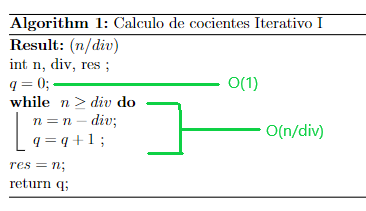
\includegraphics[width=0.7 \textwidth]{Images/A_Priori/priori_1.png}
            \caption{Analisis a Priori: Calculo de Cocientes I}
            \label{fig:priori1}
        \end{figure}
    \newpage    
    \subsection{Análisis a Priori 2}
        La figura \ref{fig:priori2} presenta el análisis a priori realizado sobre el pseudocódigo del segundo algoritmo iterativo de calculo de cocientes. Concluyendo que el algoritmo presenta una complejidad \(f(n) = O(logn)\)
        %\(f(n) = O(n)\)
        
        \begin{figure}[htp!]
            \centering
            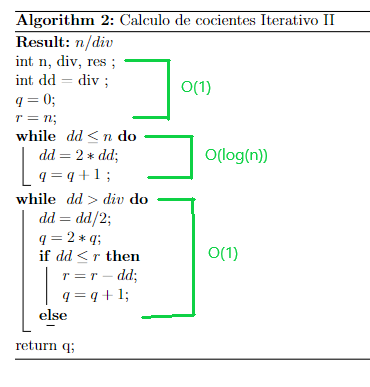
\includegraphics[width=0.7 \textwidth]{Images/A_Priori/priori_2.png}
            \caption{Analisis a Priori: Calculo de Cocientes II}
            \label{fig:priori2}
        \end{figure}
    
    \newpage
    \subsection{Análisis a Priori 3}
        La figura \ref{fig:priori3} presenta el análisis a priori realizado sobre el pseudocódigo del tercer algoritmo iterativo de calculo de cocientes. 
        \begin{figure}[htp!]
            \centering
            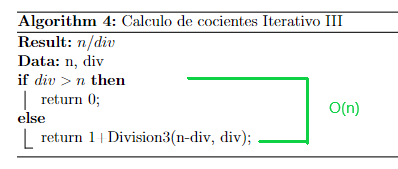
\includegraphics[width=0.7 \textwidth]{Images/A_Priori/priori_3.png}
            \caption{Analisis a Priori: Calculo de Cocientes III}
            \label{fig:priori3}
        \end{figure}
        Resolviendo 
        \begin{gather*}
            T(n) = T(n - div)+O(1)\\
            T(n) = T(n - div) + c
        \end{gather*}
        Aplicando sustitución hacia atrás:
        \begin{gather*}
            T(n)= [T(n - 2div)+c]+c\\
            T(n) = T(n - 2div)+2c
        \end{gather*}
        Donde div = i, n-i = 0, i=n
        \begin{gather*}
            T(n)=T(n-i)+ic\\
            T(n)=T(0)+nc\\
            \therefore  T(n)\in O(n)
        \end{gather*}

    
    \newpage    
    \subsection{Análisis a Posteriori 1}
        En el análisis posteriori se verifica el análisis a priori, efectivamente pudimos concluir que el cálculo de cocientes presenta tanto una complejidad lineal como logarítmica para sus diferentes casos. Para la gráfica mostrada a continuación (figura \ref{fig:posteriori1}) se muestran 1000 elementos graficados.
        \begin{figure}[htp!]
            \centering
            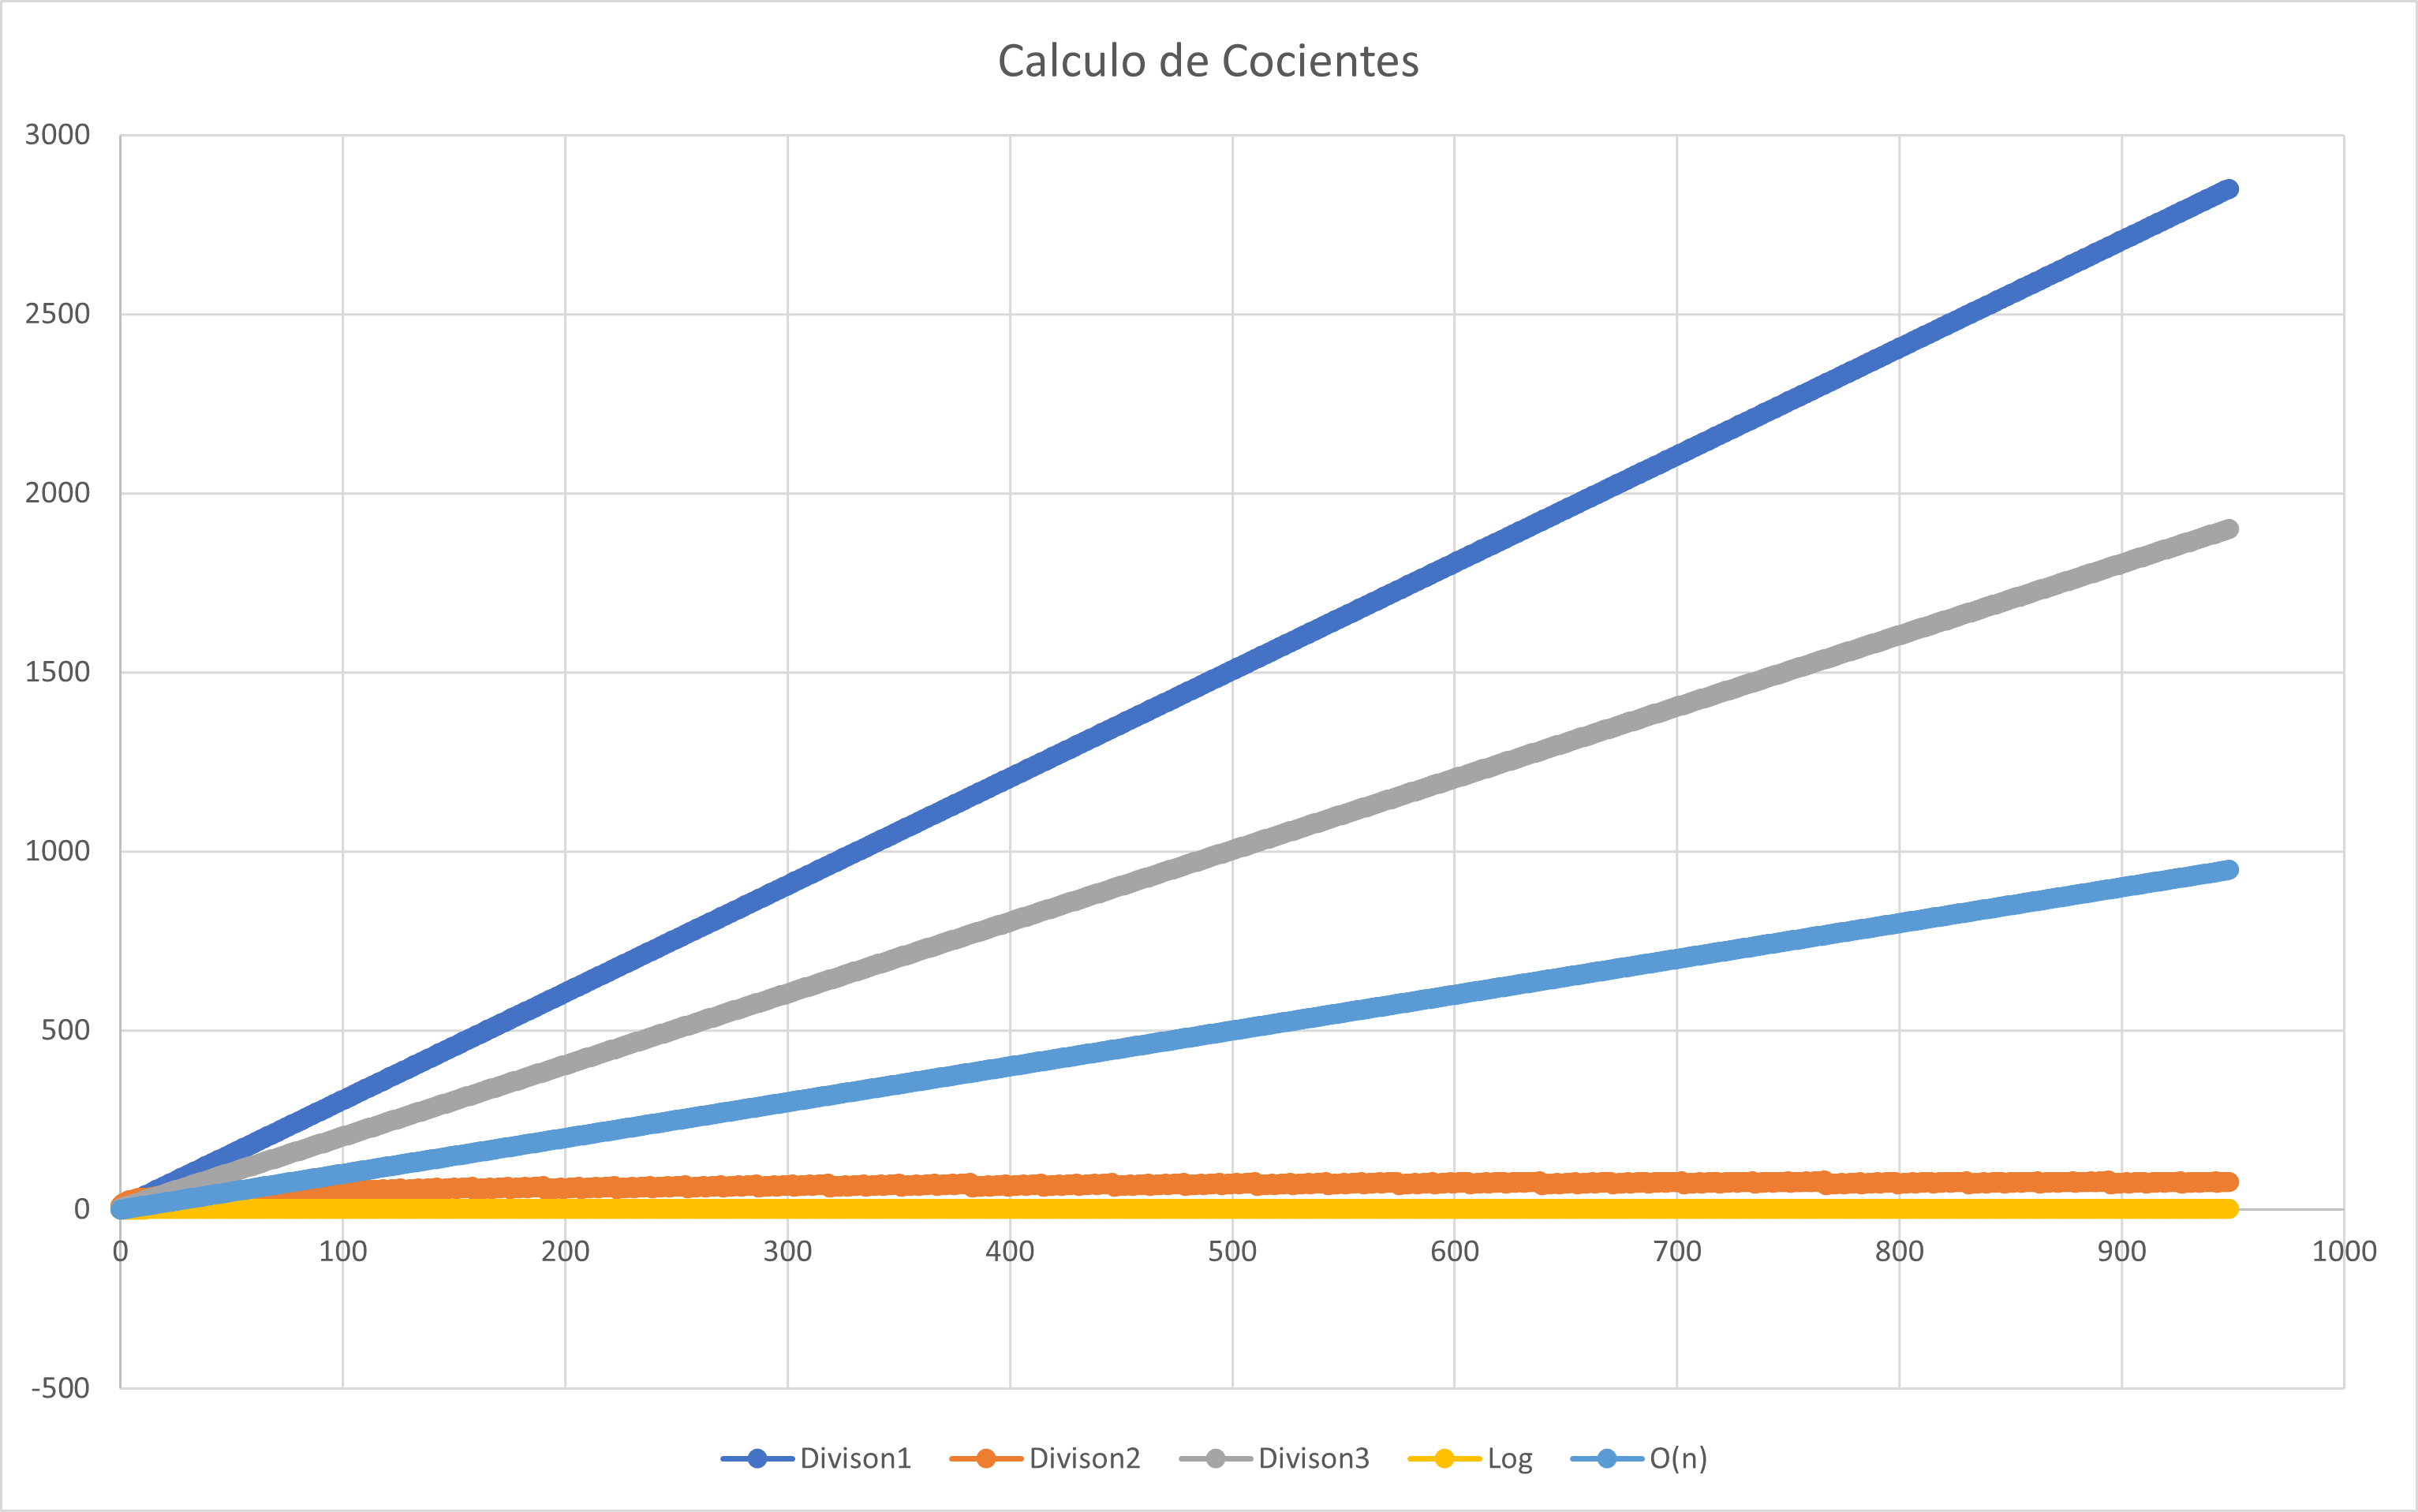
\includegraphics[width=1 \textwidth]{Images/A_Posteriori/posteriori1.png}  
            \caption{Análisis a Posteriori: Calculo de Cocientes}
            \label{fig:posteriori1}
        \end{figure}
    
    
    
    
    \newpage
    \section{Algoritmos Búsqueda Terciaria (iterativo y recursivo)}
        El algoritmo codificado en \textit{Python} fue testeado en un entorno virtual de Linux, mientras que el análisis a priori se realizó sobre los pseudocódigos.
    
    \subsection{Análisis a Priori 4}
        La figura \ref{fig:priori4} presenta el análisis a priori realizado sobre el pseudocódigo del  primer algoritmo de búsqueda terciaria. Concluyendo que el algoritmo presenta una complejidad \(f(n) = O(logn)\)
        %\(f(n) = O(n)\)
        
        \begin{figure}[htp!]
            \centering
            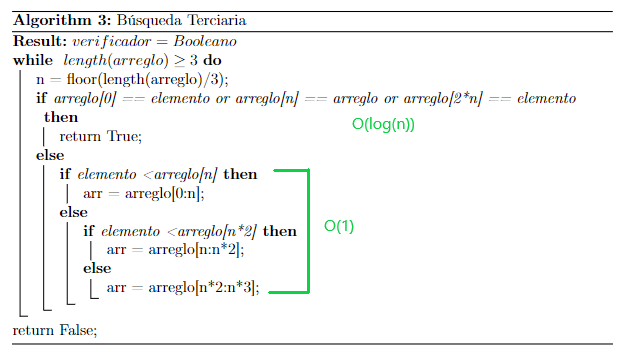
\includegraphics[width=0.7 \textwidth]{Images/A_Priori/priori_4.png}
            \caption{Analisis a Priori: Búsqueda Terciaria Iterativo}
            \label{fig:priori4}
        \end{figure}
    
    \newpage
    \subsection{Análisis a Priori 5}
        La figura \ref{fig:priori5} presenta el análisis a priori realizado sobre el pseudocódigo del segundo algoritmo de búsqueda terciaria.
        \begin{figure}[htp!]
            \centering
            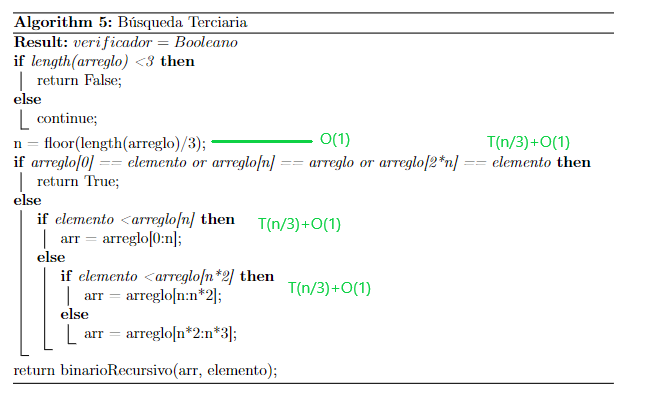
\includegraphics[width=0.7 \textwidth]{Images/A_Priori/priori_5.png}
            \caption{Analisis a Priori: Búsqueda Terciaria Recursivo}
            \label{fig:priori5}
        \end{figure}
        Resolviendo 
        \begin{gather*}
            T(n) = T(n/3)+O(1)\\
            T(n) = T(n/3) + c
        \end{gather*}
        Aplicando sustitución hacia atrás dónde n = 3 y k = logn:
        \begin{gather*}
            T(n)= T(3^{k-1})+c\\
            T(n)= [T(3^{k-1})+c]+c\\
            T(n)= T(3^{k-1})+2c
        \end{gather*}
        Donde k-1 = 0, i=k
        \begin{gather*}
            T(n)= T(3^{k-i})+ic\\
            T(n)= T(3^{0})+kc\\
            T(n)= c + c\log_3 n\\
            \therefore  T(n)\in O(\log n)
        \end{gather*}

    
    \newpage    
    \subsection{Análisis a Posteriori 2}
        En el análisis posteriori del algoritmo en su forma iterativa y recursiva, en las figuras \ref{fig:posteriori2} y \ref{fig:posteriori3} se verifica que el grado de complejidad de ambos algoritmos es el mismo, \(f(n) = O(logn)\), siendo que su complejidad aumenta en gran medida mediante más elementos aleatorios se introducen.
        \begin{figure}[htp!]
            \centering
            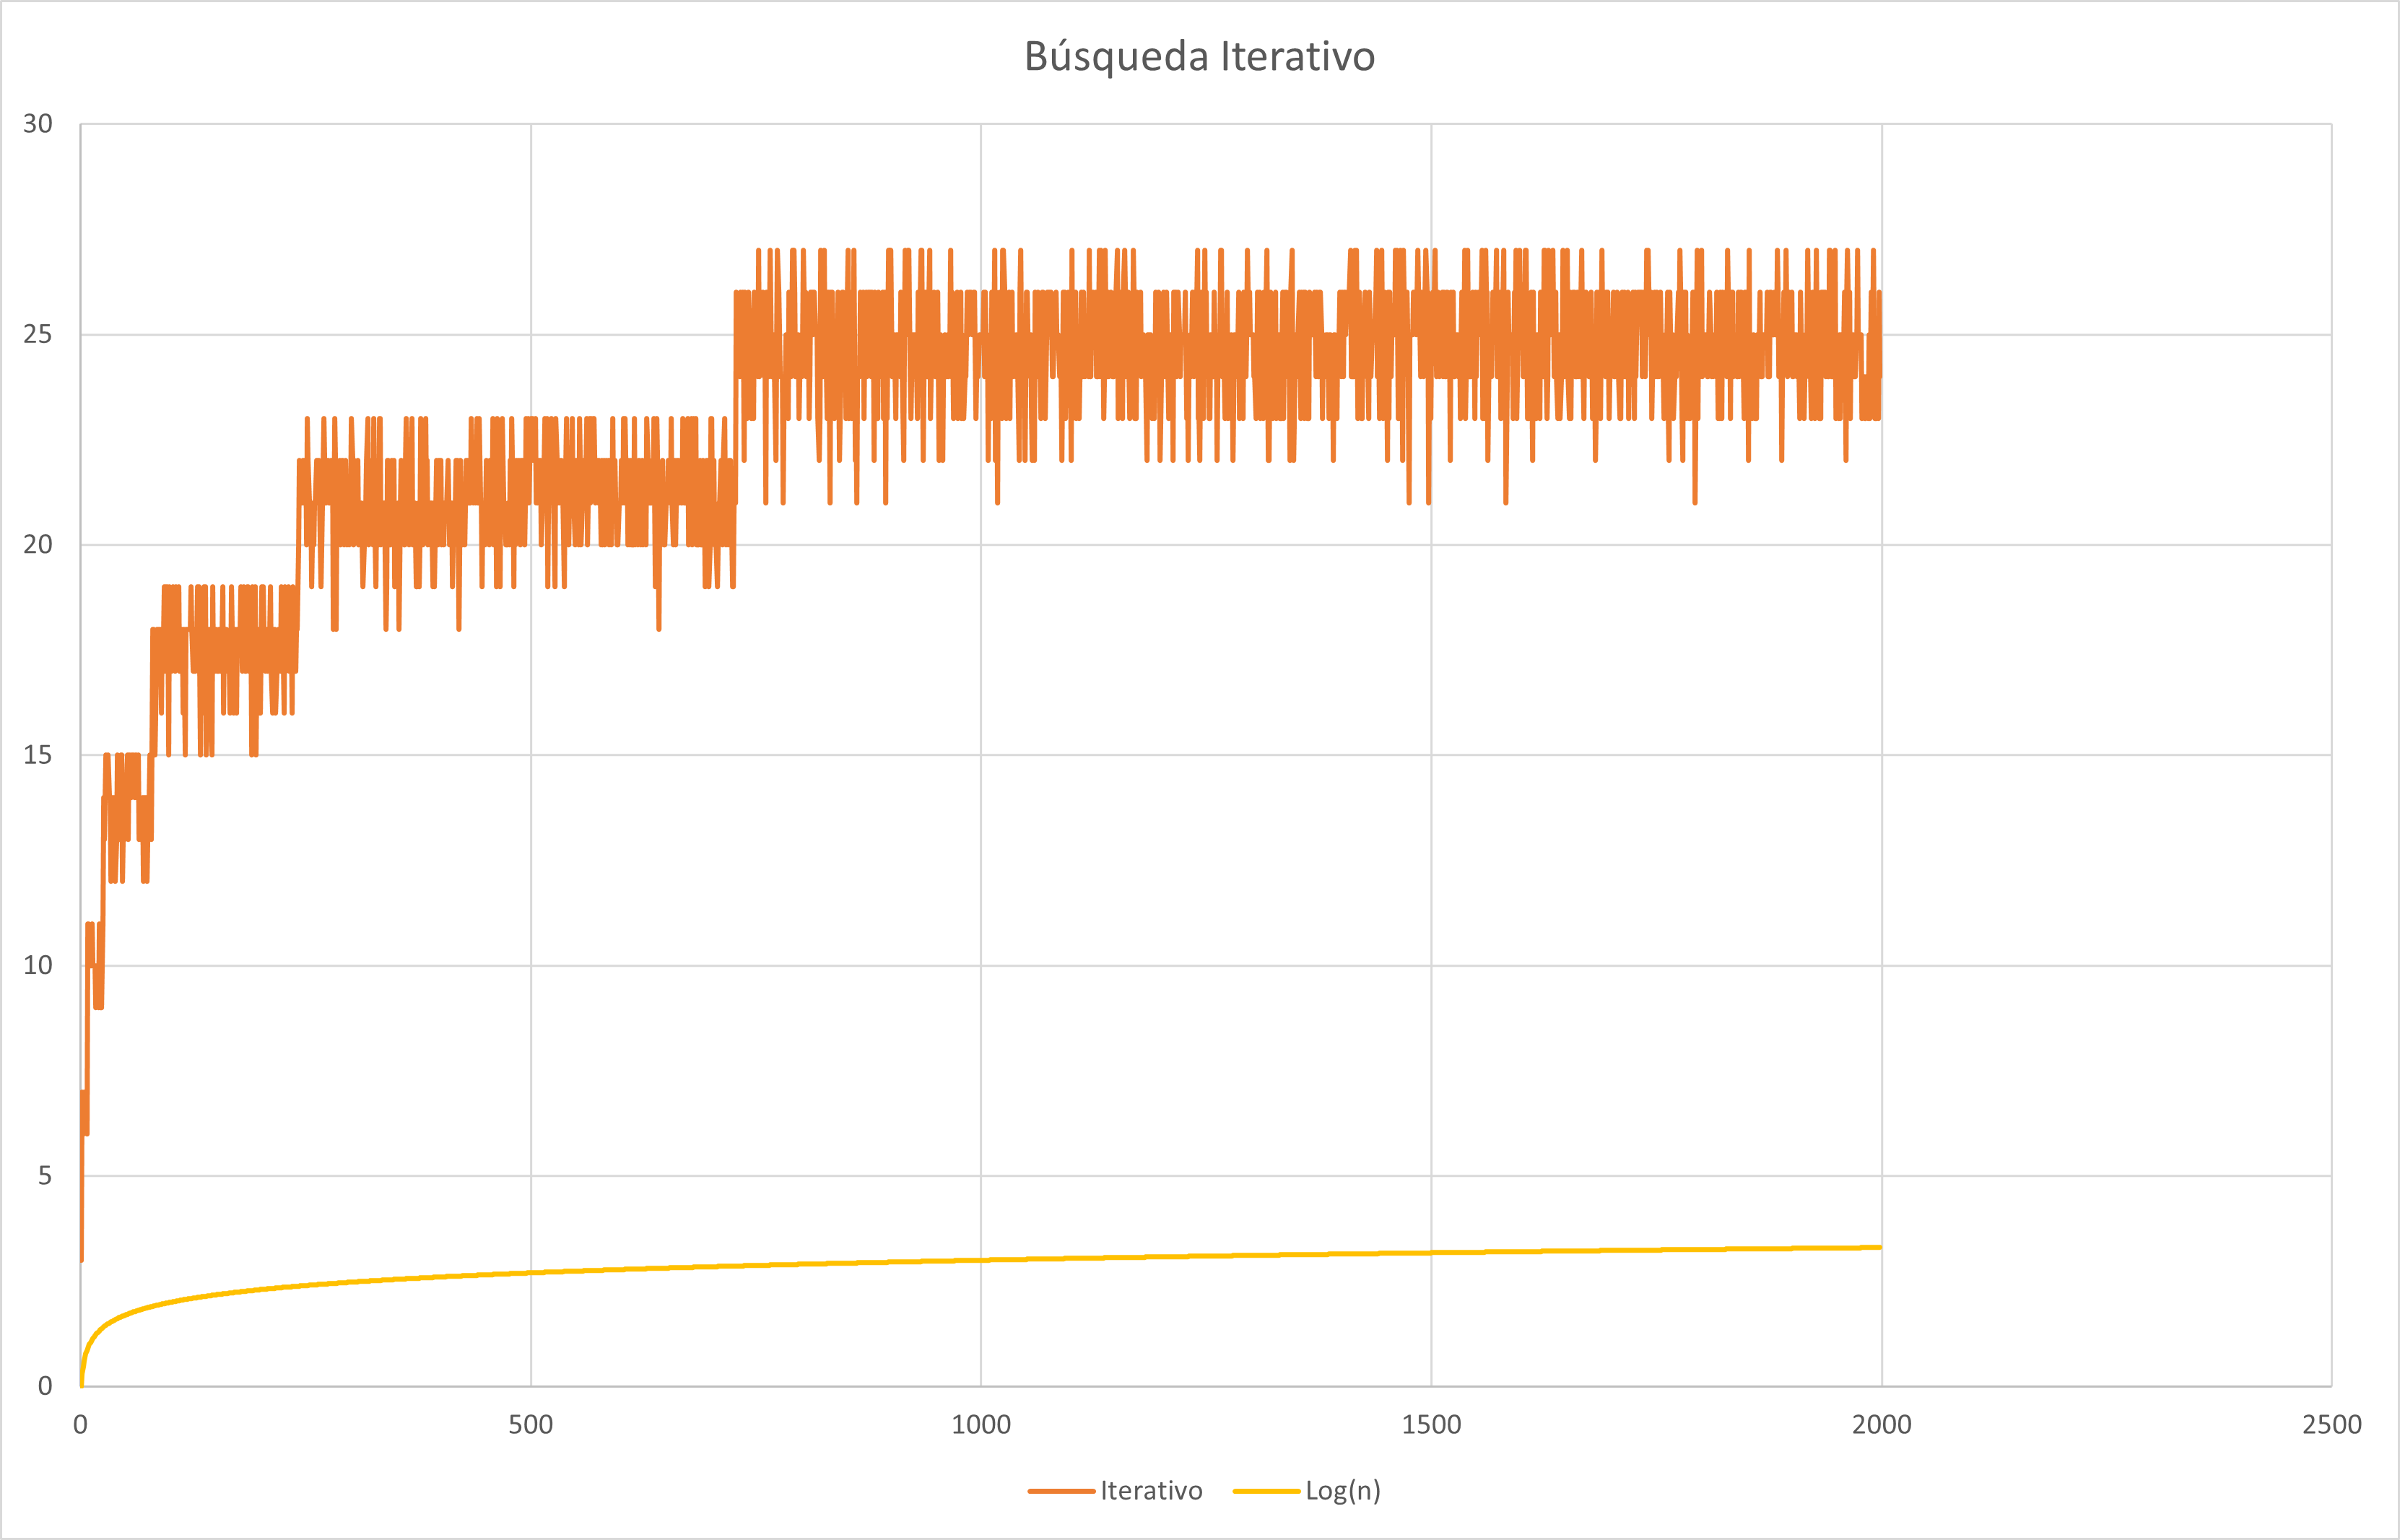
\includegraphics[width=0.8 \textwidth]{Images/A_Posteriori/posteriori2.png}  
            \caption{Análisis a Posteriori: Búsqueda Terciaria Iterativo}
            \label{fig:posteriori2}
        \end{figure}
        
        \begin{figure}[htp!]
            \centering
            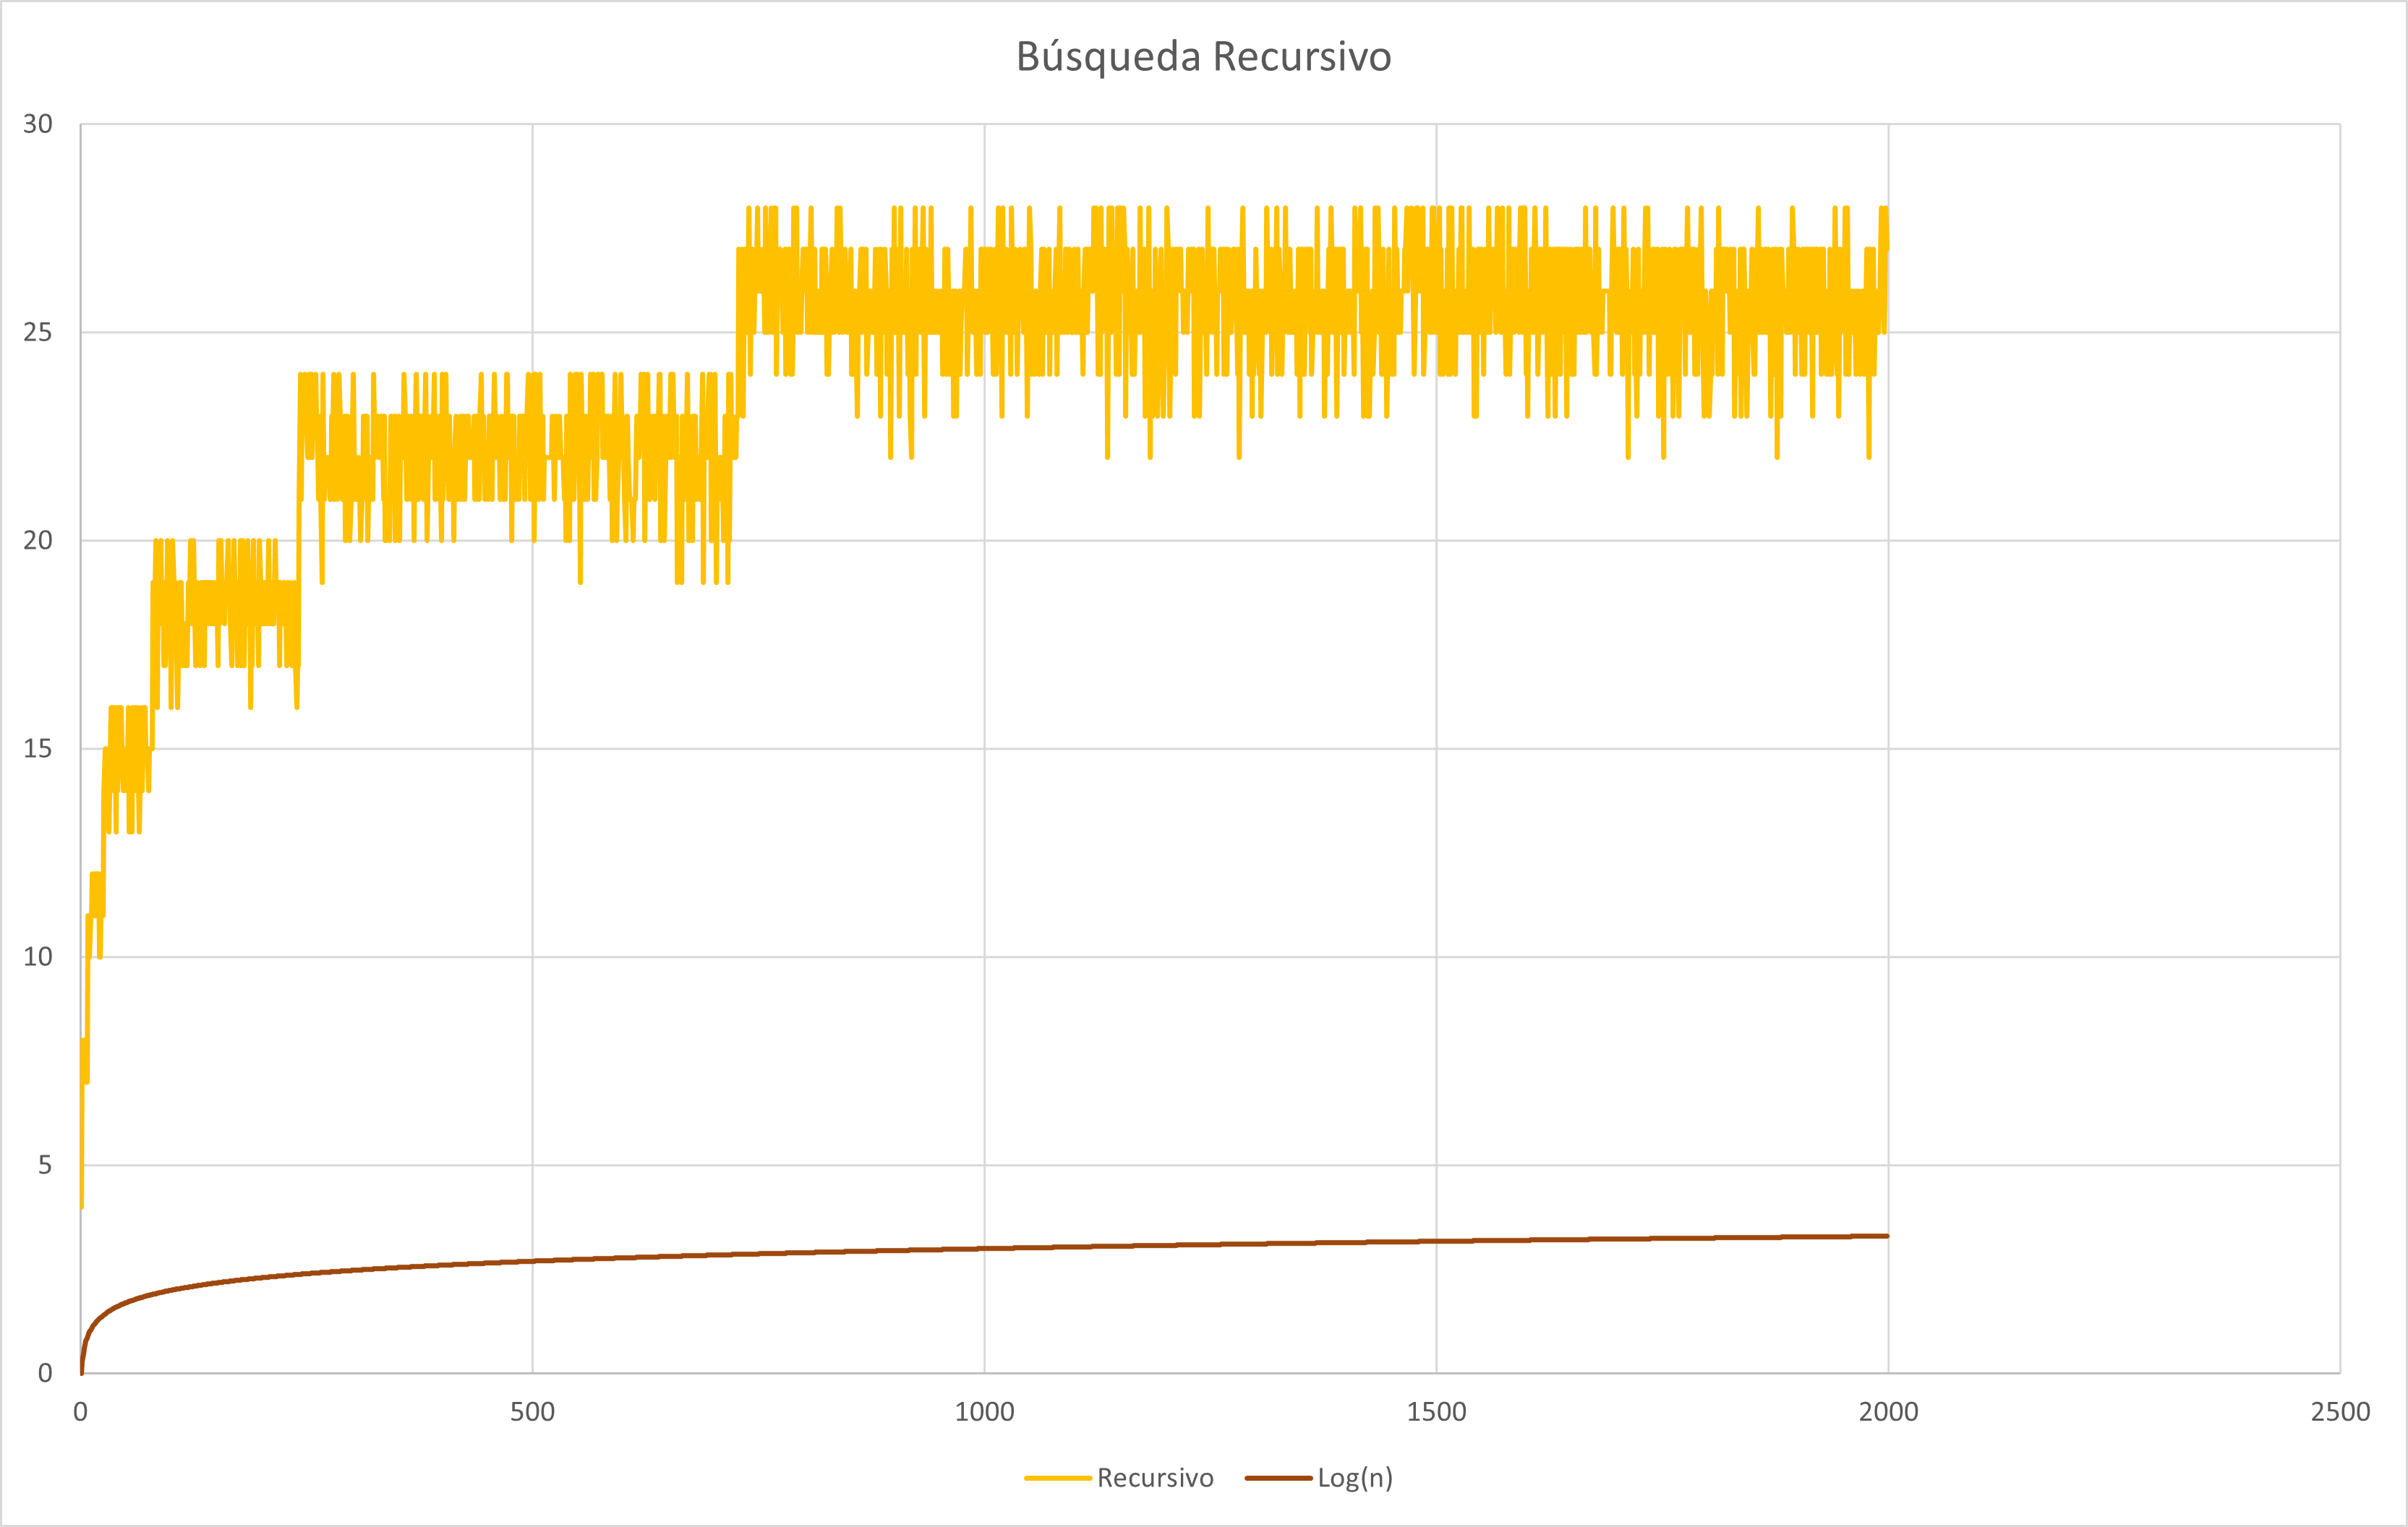
\includegraphics[width=0.8 \textwidth]{Images/A_Posteriori/posteriori3.png}  
            \caption{Análisis a Posteriori: Búsqueda Terciaria Recursivo}
            \label{fig:posteriori3}
        \end{figure}
    \newpage    
    \section{Pantallas de Ejecución de Algoritmos}
    Se muestra en las figura \ref{fig:cocientes} y \ref{fig:busq} la ejecución de los algoritmos. 
    En la figura \ref{fig:cocientes}  se puede observar la ejecución de los 3 algoritmos del cálculo de cocientes en un solo script de \textit{Python}. 
    Mientras que en la figura \ref{fig:busq} se observa la ejecución de ambos algoritmos de búsqueda terciaria. En la terminal los resultados son compuestos por la longitud de n para el arreglo y ambos tiempos de ejecución. 
    
        \begin{figure}[htp!]
            \centering
            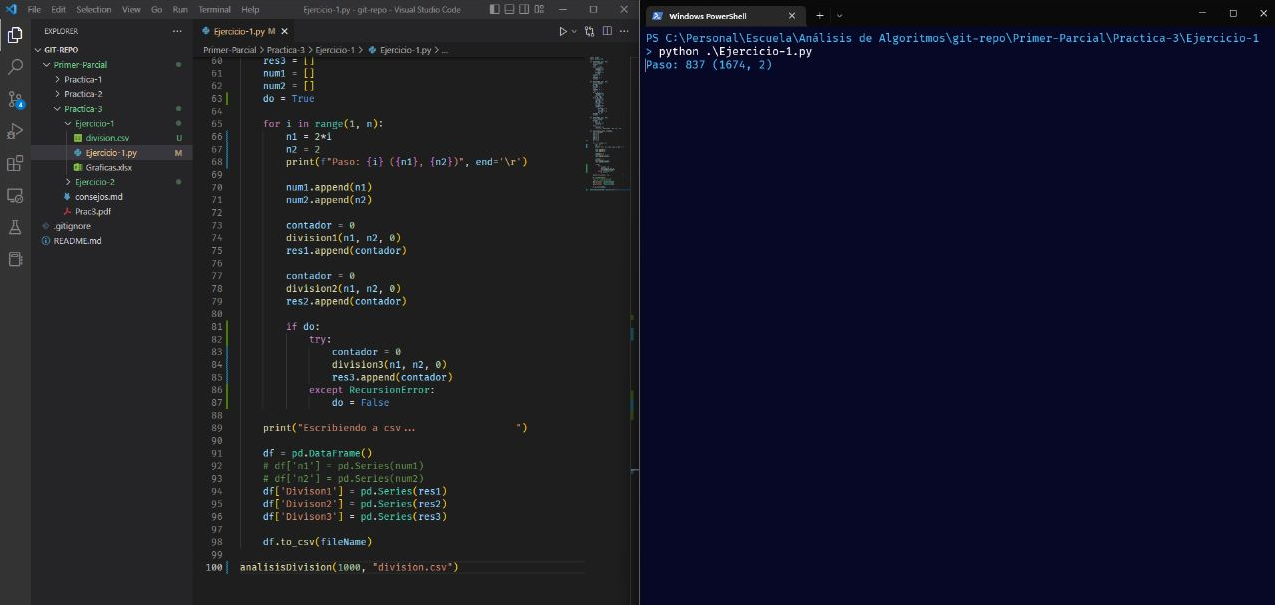
\includegraphics[width=0.8 \textwidth]{Images/Pantallas/pantalla1.png}  
            \caption{Ejecución de Calculo de Cocientes}
            \label{fig:cocientes}
        \end{figure}
        
        \begin{figure}[htp!]
            \centering
            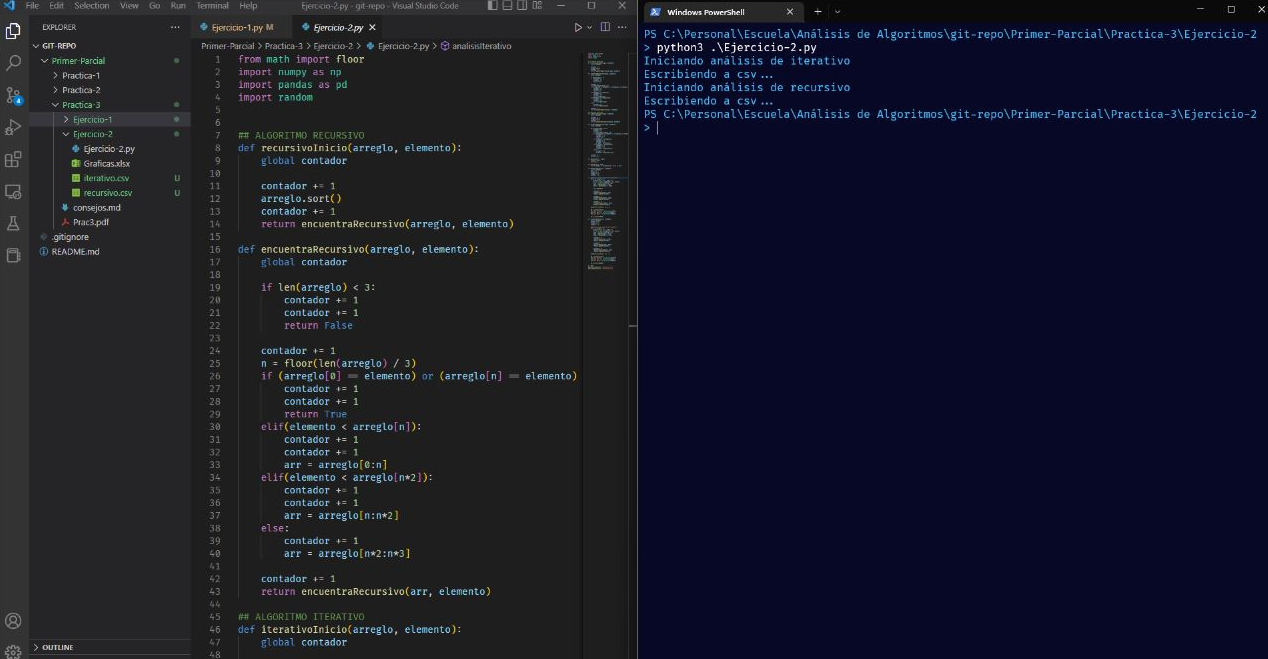
\includegraphics[width=0.8 \textwidth]{Images/Pantallas/pantalla2.png}  
            \caption{Ejecución de Búsqueda Terciaria}
            \label{fig:busq}
        \end{figure}
